\chapter{Ground Segment}

\section{Overview}

The ground segment comprises those elements of the space mission that are used to control the spacecraft and its payload, and to process the data returned from it. The activities can be divided into two general domains: control and monitoring of the spacecraft platform, and operation and exploitation of the payload.

\section{Ground Station System}

For everything related to the space link (i.e. that radio communications path between ground and space segment), the standards presented in section \ref{sec:Space Link} apply.

\begin{tabular}{l}
\textit{"Ground Equipment Monitoring Service (GEMS)" \cite{XXXXX}} \\
\end{tabular}

The GEMS specification defines a standard, platform independent model (PIM) for controlling a wide range of devices used as ground station equipment. The GEMS model does not presume or try to define a specific system level architecture. Instead, it defines generic concepts such as devices, parameters, and directives that are relatively simple to implement and provide system integrators common ways to control heterogeneous suites of space related ground equipment. The central concept of GEMS is the GEMS device. GEMS devices have typed parameters, accept directives with typed arguments, and can optionally save and restore their configuration using persistent storage. Users utilize the GEMS interface within the device to configure and obtain status.

The specification defines a simple ASCII message protocol usable across a variety of transport mechanisms, including networks, serial lines and internal data buses. The message structure is human-readable and easy to process.

\section{Ground Communications System}

\begin{tabular}{l}
\textit{CCSDS 910.0-G "Space Link Extension Services - Executive Summary" \cite{CCSDS-910.0-G}} \\
\textit{CCSDS 910.3-G "Cross Support Concept — Part 1:  Space Link Extension" \cite{CCSDS-910.3-G}} \\
\textit{CCSDS 910.4-B "Cross Support Reference Model—Part 1: Space Link Extension Services" \cite{CCSDS-910.4-B}} \\
\end{tabular}

The space link extension (SLE) services extend the return telemetry (TM) and forward telecommand (TC) space link services (see \ref{sec:Space Link} and \ref{fig:Domain of Space Link and Space Link Extension Services}) in terms of: over (ground) distance, in time, and/or by adding information.

\begin{figure}[h]
\centering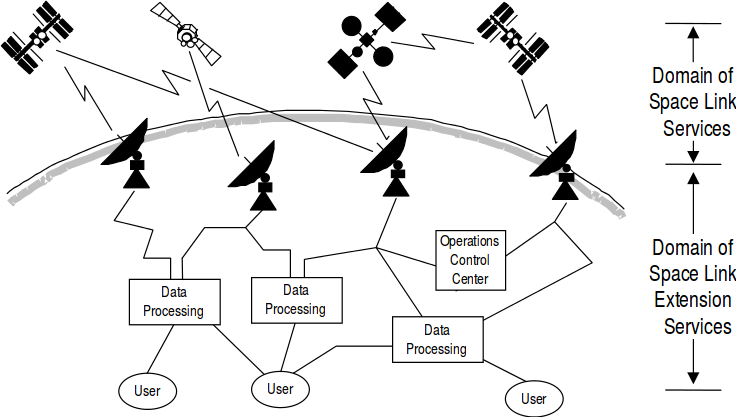
\includegraphics[scale=0.5]{fig/domains_of_space_link_and_space_link_extension_services}
\caption{Domain of Space Link and Space Link Extension Services}
\label{fig:Domain of Space Link and Space Link Extension Services}
\end{figure}

The SLE services include two major elements:

\begin{itemize}
\item data transfer services that move space link data units between ground stations, control centers, and end-user facilities;
\item management services that control the scheduling and provisioning of the transfer services.
\end{itemize}

The SLE services operate in two phases:

\begin{itemize}
\item the definition phase, when most of the management activities take place;
\item the utilization phase, when the data transfer takes place (this can be either in real-time or off-line with respect to the contact time with the spacecraft).
\end{itemize}

The adherence to SLE standards makes it possible to implement cross support among ground station providers and satellite operators. Due to the well defined SLE interfaces and functionality if SLE elements, a large number of different cross support scenarios are feasible. For example, Figure \ref{fig:Multiple Limited Capability Ground Stations} illustrates the case in which multiple minimal ground stations each send all frames received during a pass to a single complex. This complex performs all the remaining return processing and distributes the data to users. Similarly, this complex accepts forward data from users, processes it, and transmits it to the ground stations for transmission to the mission spacecraft.

\begin{figure}[h]
\centering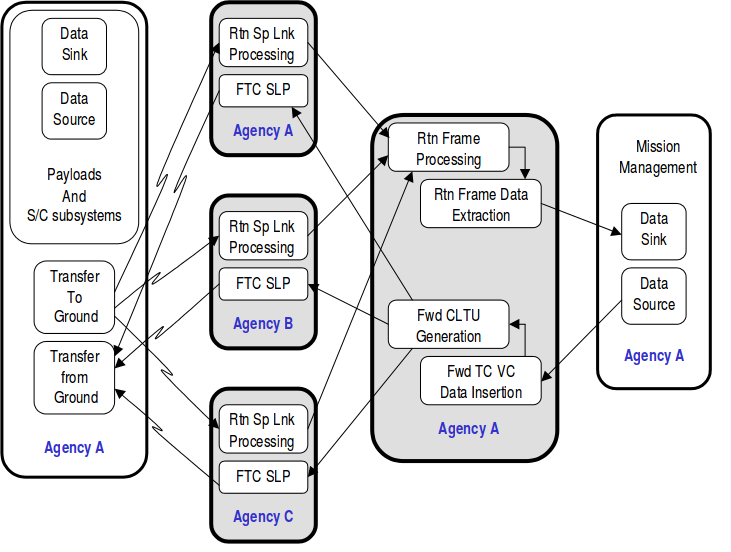
\includegraphics[scale=0.5]{fig/multiple_limited_capability_ground_stations}
\caption{Multiple Limited Capability Ground Stations}
\label{fig:Multiple Limited Capability Ground Stations}
\end{figure}

\subsection{SLE Service Management}

\begin{tabular}{l}
\textit{CCSDS 910.14-G "Space Communication Cross Support — Service Management — Operations Concept" \cite{CCSDS-910.14-G}} \\
\textit{CCSDS 910.11-B "Space Communication Cross Support — Service Management — Service Specification" \cite{CCSDS-910.11-B}} \\
\end{tabular}

Although the SLE data transfer services can be implemented with an ad-hoc (user agreed) service management, adhering to the SLE service management standard provides a formal and clear definition of services for negotiation, configuration, and execution of space link services, and thus allows for maximum of automation of this tasks. 

The service management functions are implemented by the utilization management (UM) on the user side and the complex management (CM) on the provider side (see Figure \ref{fig:Service Management Environment}). The following four services are defined:

\begin{itemize}
\item Service package service, which addresses the arrangement of spacecraft space link session times and execution of the SLE transfer services.
\item Configuration profile service, which addresses the establishment of sets of data concerning the space link and ground station configuration.
\item Trajectory prediction service, which addresses the transfer and updating of spacecraft trajectory data.
\item Service agreement service, which addresses the information that needs to be agreed upon before a cross support service can be established.
\end{itemize}

\begin{figure}[h]
\centering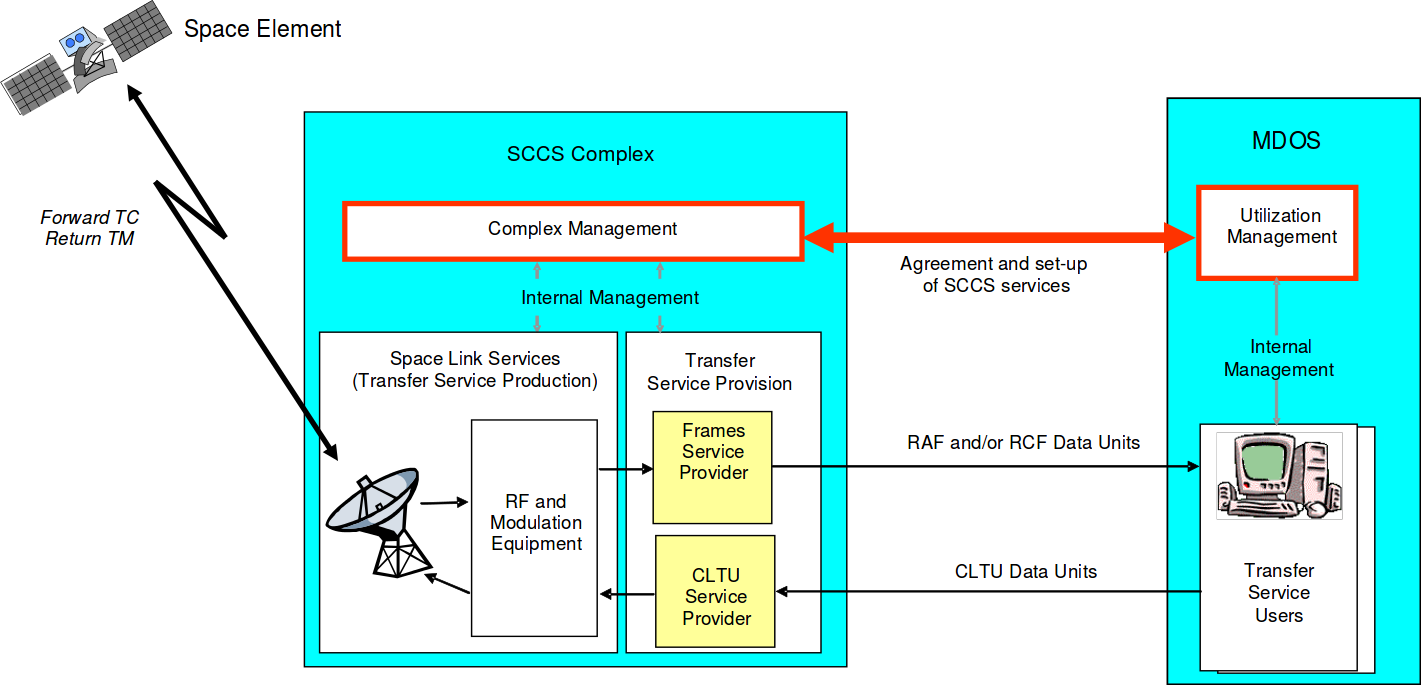
\includegraphics[scale=0.3]{fig/service_management_environment}
\caption{Service Management Environment}
\label{fig:Service Management Environment}
\end{figure}

\subsection{SLE Transfer Services}

The SLE transfer services are a suite of services that are used to transfer specific telecommand and telemetry protocol data units. The transfer services for the forward and return space link are presented in the next sections. There are three modes of delivery for SLE transfer services:

\begin{itemize}
\item complete online, where service data is delivered in the sequence received, with no data omitted (may relay on sufficient buffering capabilities);
\item timely online, where data may be omitted (deleted) if it exceeds a defined maximum delivery delay;
\item offline, where data is transported outside a real-time space link session.
\end{itemize}

\subsubsection{Return SLE Services}

\begin{tabular}{l}
\textit{CCSDS 911.1-B "Space Link Extension — Return All Frames Service Specification" \cite{CCSDS-911.1-B}} \\
\textit{CCSDS 911.2-B "Space Link Extension — Return Channel Frames Service Specification" \cite{CCSDS-911.2-B}} \\
\textit{CCSDS 911.5-B "Space Link Extension — Return Operational Control Fields Service Specification" \cite{CCSDS-911.5-B}} \\
\end{tabular}

The return SLE services (shown in Figure \ref{fig:Return SLE Services}) include: 

\begin{itemize}
\item Return all frames (RAF): provides the telemetry frames from a single space link symbol stream to spacecraft operators and other users who might need all the frames;
\item Return channel frames (RCF): provides master channel (MC) or specific virtual channels (VCs), as specified by each RCF service user;
\item Return frame secondary header (RFSH): provides MC or VC frame secondary headers (FSHs), as specified by each RFSH service user; 
\item Return operational control field (ROCF): provides MC or VC operational control fields (OCFs) channel, as specified by each ROCF service user; 
\item Return space packet (RSP): enables single users to receive packets with selected application process identifiers (APIDs) from one spacecraft VC.
\end{itemize}

\begin{figure}[h]
\centering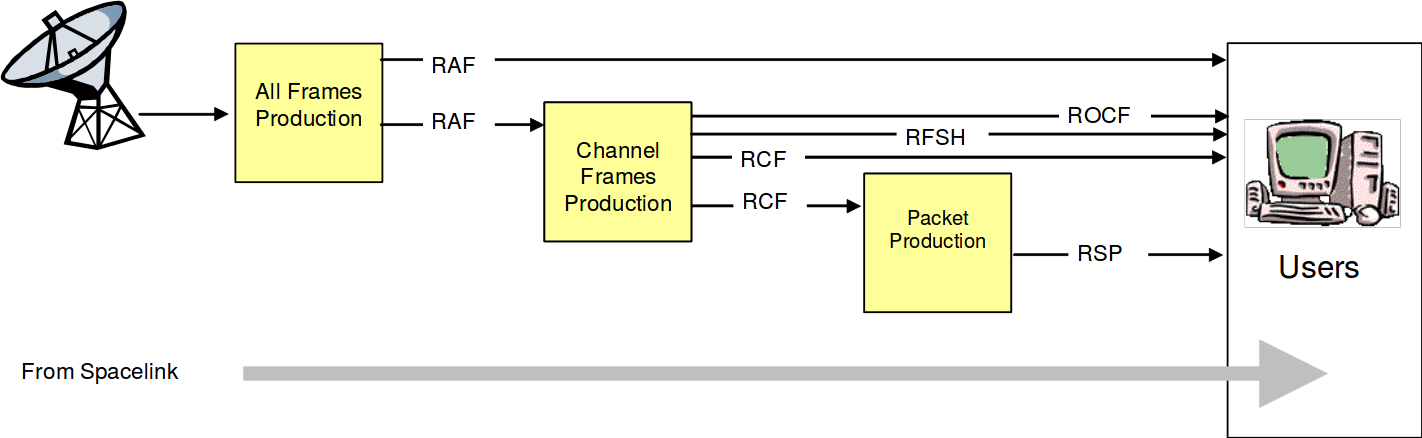
\includegraphics[scale=0.3]{fig/return_sle_services}
\caption{Return SLE Services}
\label{fig:Return SLE Services}
\end{figure}

\subsubsection{Forward SLE Services}

\begin{tabular}{l}
\textit{CCSDS 912.1-B "Space Link Extension — Forward CLTU Service Specification" \cite{CCSDS-912.1-B}} \\
\textit{CCSDS 912.3-B "Space Link Extension — Forward Space Packet Service Specification" \cite{CCSDS-912.3-B}} \\
\end{tabular}

The forward SLE services (shown in Figure \ref{fig:Forward SLE Services}) include: 

\begin{itemize}
\item Forward space packet (FSP): enables single users to provide packets for uplink to a spacecraft without needing to co-ordinate with other users of the spacecraft;
\item Forward telecommand virtual channel access (FTCVCA): enables users to provide complete VCs for uplink;
\item Forward telecommand frame (FTCF): enables users to supply TC frames to be transformed to communications link transmission units (CLTUs) ready for uplink;
\item Forward communications link transmission unit (FCLTU): enables users to provide CLTUs for pulink to the spacecraft.
\end{itemize}

\begin{figure}[h]
\centering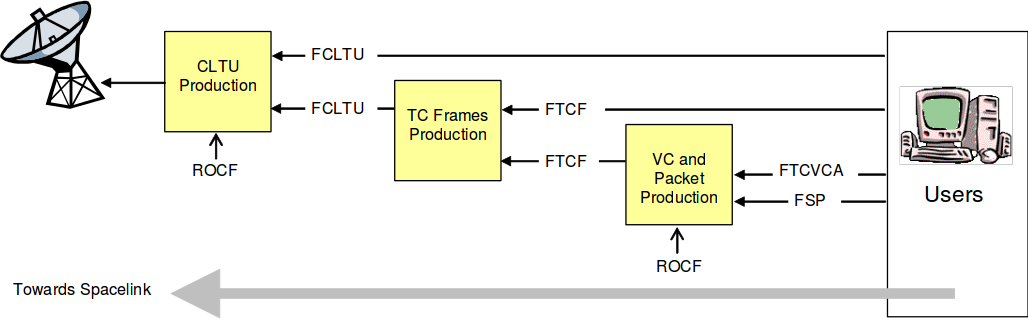
\includegraphics[scale=0.4]{fig/forward_sle_services}
\caption{Forward SLE Services}
\label{fig:Forward SLE Services}
\end{figure}

Note that as shown in Figure \ref{fig:Forward SLE Services} the ROCF service is input to the CLTU production and VC and packet production service.

\subsection{Cross Support Transfer Services}

\begin{tabular}{l}
\textit{CCSDS 921.1-R "Cross Support Transfer Service - Specification Framework" \cite{CCSDS-921.1-R}} \\
\end{tabular}

Cross support transfer services (CSTSes) provide for reliable, access-controlled transfer of spaceflight mission related data between ground element entities. A cross support service is characterized by the kind of data it transfers (e.g., telemetry data,  tracking data, service production monitoring data), and therefore different CSTSes need  to respond to specific requirements that may demand specific solutions. On the other hand, all CSTSes defined by CCSDS  apply the same basic communications patterns in order  to simplify specification, implementation, and operation of these services.  

\begin{tabular}{l}
\textit{CCSDS 922.1-R "Cross Support Transfer Service - Monitored Data Service" \cite{CCSDS-922.1-R}} \\
\end{tabular}

This standard defines a service, which allows a spaceflight mission to receive cyclic reports on, and to query the current values of, the parameters that are pertinent to cross support services being provided by a cross support complex. The service also allows a spaceflight mission to receive notifications of the occurrence of events of interest associated with the services that are being provided by the complex.

\begin{tabular}{l}
\textit{CCSDS 922.2-R "Cross Support Transfer Service - Tracking Data Cross support Transfer Service" \cite{CCSDS-922.2-R}} \\
\end{tabular}

This standard defines a service that allows a spaceflight mission to receive periodic measurements of tracking data as soon as they are generated by a cross support complex or anytime thereafter. The service delivers the tracking data formatted in accordance with the CCSDS Tracking Data Message Recommended Standard (TDM).

\subsection{API for Transfer Services}

\begin{tabular}{l}
\textit{CCSDS 914.1-G "Space Link Extension — Application Program Interface for Transfer Services — Summary of Concept and Rationale" \cite{CCSDS-914.1-G}} \\
\textit{CCSDS 914.0-M "Space Link Extension — Application Program Interface for Transfer Services — Core Specification" \cite{CCSDS-914.0-M}} \\
\textit{CCSDS 914.2-G "Space Link Extension — Application Program Interface for Transfer Services — Application Programmer's Guide" \cite{CCSDS-914.2-G}} \\
\end{tabular}

The SLE API provides a high level, communication technology independent interface for exchange of SLE operation invocations and returns between a SLE service user and a SLE service provider. 

The SLE API for transfer services consists of two distinct layers, API proxy and the API service element, shown shown in figure \ref{fig:Layers of the SLE API}.

\begin{figure}[h]
\centering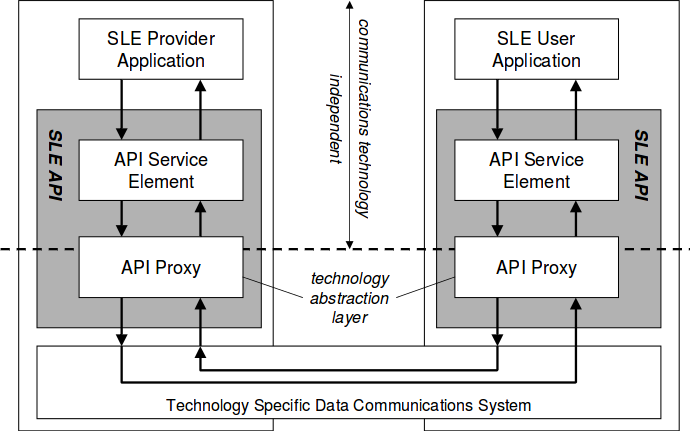
\includegraphics[scale=0.5]{fig/layers_of_the_sle_api}
\caption{Layers of the SLE API}
\label{fig:Layers of the SLE API}
\end{figure}

The API proxy represents the technology abstraction layer. 

\subsubsection{API for Return SLE Services}

\begin{tabular}{l}
\textit{CCSDS 915.1-M "Space Link Extension — Application Program Interface for Return All Frames Service" \cite{CCSDS-915.1-M}} \\
\textit{CCSDS 915.2-M "Space Link Extension — Application Program Interface for Return Channel Frames Service" \cite{CCSDS-915.2-M}} \\
\textit{CCSDS 915.5-M "Space Link Extension — Application Program Interface for Return Operational Control Fields" \cite{CCSDS-915.5-M}} \\
\end{tabular}

These standards define C++ application program interfaces (APIs) for the specified return SLE services.

\subsubsection{API for Forward SLE Services}

\begin{tabular}{l}
\textit{CCSDS 916.1-M "Space Link Extension — Application Program Interface for the Forward CLTU Service" \cite{CCSDS-916.1-M}} \\
\textit{CCSDS 916.3-M "Space Link Extension — Application Program Interface for the Forward Space Packet Service" \cite{CCSDS-916.3-M}} \\
\end{tabular}

These standards define C++ application program interfaces (APIs) for the specified forward SLE services.

\subsubsection{Internet Protocol for Transfer Services}

\begin{tabular}{l}
\textit{CCSDS 913.1-B "Space Link Extension — Internet Protocol for Transfer Services" \cite{CCSDS-913.1-B}} \\
\end{tabular}

This standard defines a protocol for transfer of SLE protocol data units (PDUs) using the internet protocols TCP (transmission control protocol) and IP (internet protocol), named internet SLE protocol one (ISP1). It is a layered protocol as shown in Figure \ref{fig:ISP1 Architectural Model}, where the:

\begin{itemize}
\item Higher layers: represent the functionality specified in the SLE transfer services;
\item Authentication layer: responsible for generating and analysing the credentials to authorize transfers;
\item Data encoding layer: responsible for encoding of SLE protocol data units received from higher layers and decoding of protocol data units received from the peer application;
\item Transport mapping layer: handles the interface to the TCP protocol.
\end{itemize}

\begin{figure}[h]
\centering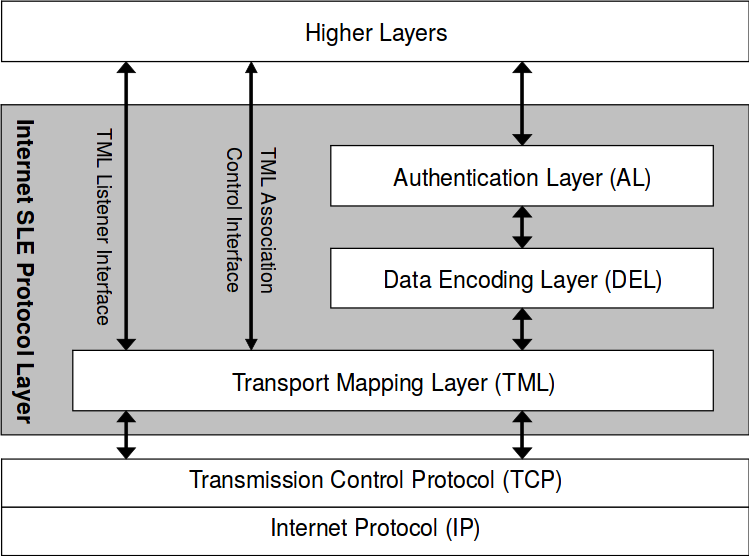
\includegraphics[scale=0.4]{fig/isp1_architectural_model}
\caption{ISP1 Architectural Model}
\label{fig:ISP1 Architectural Model}
\end{figure}

\section{Mission Operations System}

\subsection{Spacecraft Control System}

For everything related to the application layer functionality of the spacecraft control system (that is, the packet utilization standard and the CCSDS file delivery protocol), the standards presented in section \ref{sec:Onboard Software Applications} apply accordingly.

\subsubsection{Mission Information Base}

\begin{tabular}{l}
\textit{CCSDS 660.0-B "XML Telemetric and Command Exchange (XTCE)" \cite{CCSDS-660.0-B}} \\
\textit{CCSDS 660.0-G "XML Telemetric and Command Exchange (XTCE)" \cite{CCSDS-660.0-G}} \\
\textit{CCSDS 660.1-G "XML Telemetric and Command Exchange (XTCE) - Element Description" \cite{CCSDS-660.1-G}} \\
\end{tabular}

XTCE is a solution to specify and exchange telemetry and telecommand databases in an open, non-proprietary way using XML. The main concept behind XTCE is that of a hierarchy of information. Hence XTCE can be applied to any part of the spacecraft (such as instruments), the spacecraft itself, or the entire space or ground segment. Typically, individual databases would be created for each payload and for the spacecraft platform itself, which then can be integrated into one large database. 

\subsubsection{Monitoring and Control Data}

\begin{tabular}{l}
\textit{ECSS-E-ST-70-31 "Ground systems and operations - Monitoring and control data definition" \cite{ECSS-E-ST-70-31}} \\
\end{tabular}

The purpose of this specification is to define the data that is associated with the monitor and control of system elements (that are referred to as products). It defines \textsl{what} is to be provided rather then \textsl{how}.

A product consists of hardware component, software component, or both, together with associated documentation containing all the product knowledge. To facilitate the sharing and reuse of the product knowledge, this standards defines a formal structure, named the space system model (SSM). An example of the SSM of a product is shown in figure \ref{fig:Example Product Delivery System Element Hierarchy}.

\begin{figure}[h]
\centering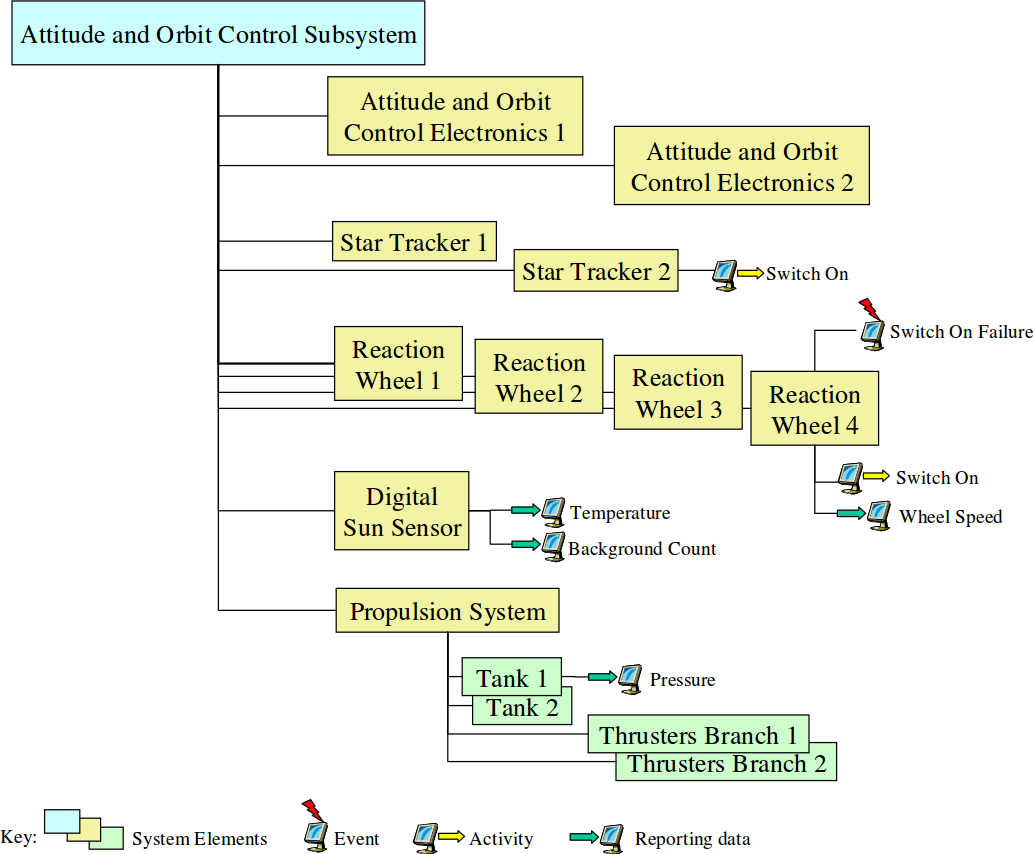
\includegraphics[scale=0.35]{fig/example_product_delivery_system_element_hierarchy}
\caption{Example Product Delivery System Element Hierarchy}
\label{fig:Example Product Delivery System Element Hierarchy}
\end{figure}

The SSM simply consists of:
\begin{itemize}
\item "Entity" types, e.g. system elements
\item "Value" types, e.g. an application program identifier (APID)
\end{itemize}

The SSM types that are relevant for monitoring and control purposes are system elements and their associated activities, reporting data, events, and constituent system elements.

The \textbf{system elements} correspond to the elements of the space system resulting from the functional decomposition.

An \textbf{activity} is a space system monitoring and control function implemented within the ground support equipment or mission control system. An activity can be implemented as a telecommand either to the space segment or to the ground segment, a procedure, an operating system command (e.g. a printer request, sending an email, transferring a file using FTP) or any other command type that is specific to a given implementation of the space system (e.g. a command to a special check-out system or to a ground station).

\textbf{Reporting data} is information that a system element provides, irrespective of how this information is used. Reporting data can comprise measurements which reflect the state of the associated system element or an output product whose purpose is to be used by another system element (e.g. manoeuvre parameters provided by the flight dynamics system). Reporting data comprises parameters and compound parameters. A parameter is the lowest level of elementary information that has a meaning for monitoring and control of the space system. A compound parameter is a record comprised of any sequence of parameters, arrays of parameters and sub-records. For example, a complete telemetry packet, or part thereof, may be represented as a compound parameter. The parameters within a compound parameter are normally interpreted together. Reporting data can have different representations depending on its life cycle within the space system (e.g. an on-board measurement has a raw value in telemetry and an engineering value when presented on a ground segment display).

An \textbf{event} is an occurrence of a condition or group of conditions of operational significance. Events are widely used within the space system to trigger the execution of functions (e.g. acquisition of signal can initiate telemetry processing tasks at the ground station). Users can define mission-specific events, associated with a system element, for example for use within procedures.

\subsection{Operations Management System}

\subsubsection{Procedures}

\begin{tabular}{l}
\textit{ECSS-E-ST-70-32 "Test and operations procedure language" \cite{ECSS-E-ST-70-32}} \\
\end{tabular}

A procedure is the principle mechanism to control the space system during pre-launch functional testing and post-launch in-orbit operations. There are two types of flight control procedures (FCP):

\begin{itemize}
\item \textbf{Nominal procedures}: These define the set of in-orbit operations of the space system to be used under nominal conditions. They constitute the building blocks from which the mission timelines and schedules of the flight operations plan (FOP) are constructed. 
\item \textbf{Contingency procedures}: These define the recovery actions used to reconfigure the space system if pre-identified anomalies or failures occur.
\end{itemize}

Although FCPs have traditionally been executed under manual control, pressure to reduce manpower during routine mission operations implies more automation of routine tasks such as the execution of procedures.

This standard defines a reference language, named "procedure language for users in test and operations (PLUTO)" for constructing FCPs for manual and/or automated execution.

A PLUTO procedure comprises the following elements (Figure \ref{fig:Example of PLUTO Procedure}):

\begin{itemize}
\item An optional declaration body, which declares the local events that can be raised within the procedure. 
\item An optional preconditions body, which ensures that the procedure is only executed if (or when) pre-defined initial conditions are satisfied.
\item A mandatory main body, which fulfills the goal of the procedure. The main body can be composed of self-contained sub-goals fulfilled by activities or steps.
\item An optional watchdog body, which manages contingency situations that can arise during the execution of the procedure. The watchdog body is composed of one or more special steps, called watchdog steps, which are all initiated in parallel.
\item An optional confirmation body, which assesses whether the objectives of the procedure have been achieved or not. 
\end{itemize}

 \begin{figure}[h]
\centering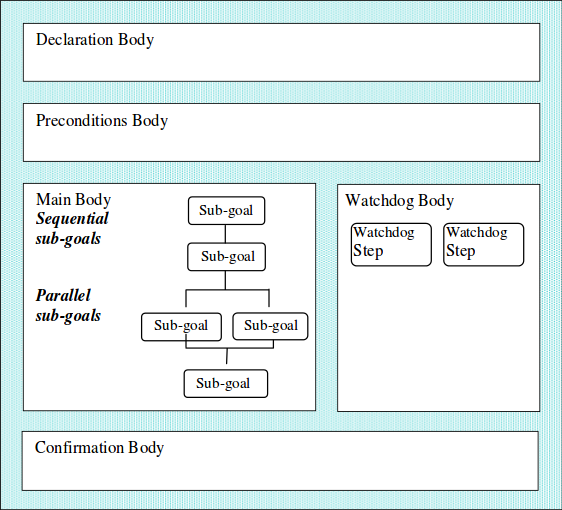
\includegraphics[scale=0.45]{fig/example_of_pluto_procedure}
\caption{Example of PLUTO Procedure}
\label{fig:Example of PLUTO Procedure}
\end{figure}

\subsubsection{Mission Planning}

\begin{tabular}{l}
\textit{CCSDS 902.1-R "Simple Schedule Format Specification" \cite{CCSDS 902.1-R}} \\
\end{tabular}

This standard specifies a standard format for use in transferring scheduling information related to ground stations and/or relay satellites between spacecraft operators. The schedule is an XML file that contains information about the times that one or more ground stations have been booked for tracking one or more satellites.

\subsubsection{Data Archival and Dissemination System}

\begin{tabular}{l}
\textit{CCSDS 661.0-B "XML Formatted Data Unit (XFDU) Structure and Construction Rules" \cite{CCSDS 661.0-B}} \\
\end{tabular}

This standard defines a technique for the packaging of data and metadata, including software, into a single package (e.g., file or message) to facilitate information transfer and archiving. It provides a detailed specification of core packaging structures and mechanisms to accommodate the current computing environment and meet evolving requirements by making the packaging manifest an XML document defined by the XML Schema specified in the document.

\begin{tabular}{l}
\textit{CCSDS 650.0-M "Reference Model for an Open Archival Information System (OAIS)" \cite{CCSDS 650.0-M}} \\
\textit{CCSDS 651.0-M "Producer-Archive Interface Methodology Abstract Standard" \cite{CCSDS 651.0-M}} \\
\textit{CCSDS 651.1-B "Producer-Archive Interface Specification (PAIS)" \cite{CCSDS 651.1-B}} \\
\end{tabular}

The Open Archival Information System (OAIS) is a reference model rather than an implementation plan for a long term digital archive. As a conceptual framework for a complete, generic archival system, OAIS's strength is in establishing common terms and concepts for describing repository architectures and comparing implementations — without specifying an implementation an organization should use. 

The OAIS environment is derived from the interaction of four entities: producers, consumers, management and the archive itself. Producers supply the information that the archive preserves. Consumers use the preserved information. A special class of consumers is the Designated Community - the subset of consumers who are expected to understand the archived information. Management is the entity responsible for establishing the broad policy objectives of the archive (e.g. determining what types of information are to be archived, identifying funding sources, etc.). The management entity does not include the day-to-day administration of the archive; this task is performed by a functional entity within the archive itself.

Within the OAIS entity, five functional units are identified (shown in Figure \ref{fig:OAIS Functional Entities}).

\begin{figure}[h]
\centering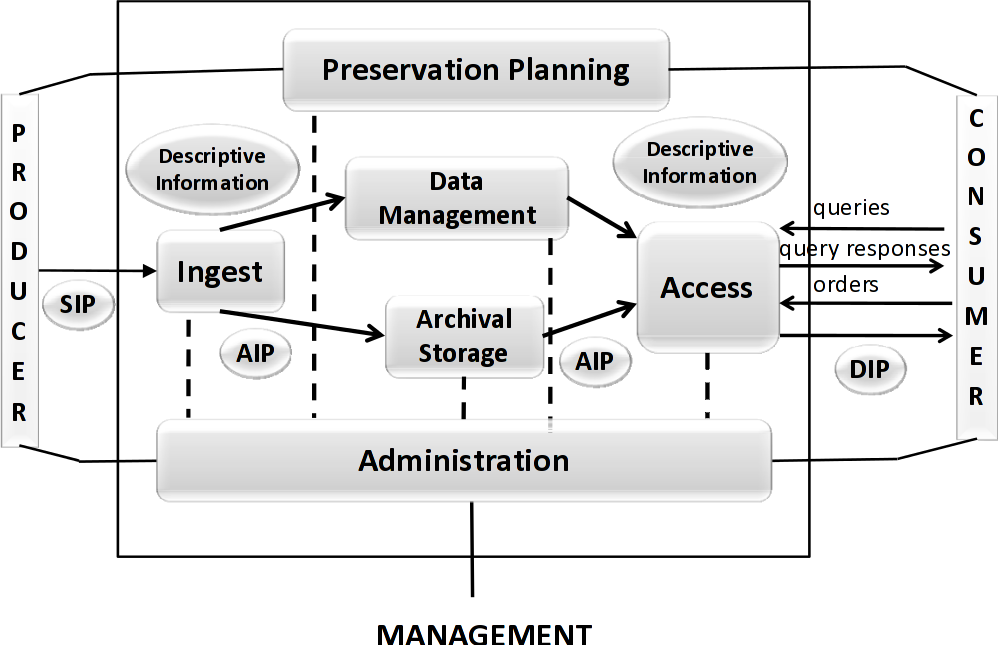
\includegraphics[scale=0.35]{fig/oais_functional_entities}
\caption{OAIS Functional Entities}
\label{fig:OAIS Functional Entities}
\end{figure}

The \textbf{Ingest} function is responsible for receiving information from producers and preparing it for storage and management within the archive. More specifically, the Ingest entity accepts information from producers in the form of SIPs, performs quality assurance checks on the SIP, generates an AIP from one or more SIPs and extracts Descriptive Information from the AIPs (metadata for search and retrieval, thumbnail images for browsing, etc.). Finally, the Ingest function transfers the newly created AIPs to Archival Storage and the associated Descriptive Information to Data Management.

The \textbf{Archival Storage} function handles the storage, maintenance and retrieval of the AIPs held by the archive. These responsibilities include receiving new AIPs from the Ingest function and assigning them to permanent storage according to various criteria (media requirements, expected utilization rates, etc.), migrating AIPs to new media as required, error checking, implementing disaster recovery strategies, and providing copies of requested AIPs to the Access function.

The \textbf{Data Management} function coordinates the Descriptive Information pertaining to the archive's AIPs, in addition to system information used in support of the archive's operation. In particular, the Data Management function maintains and administers the database containing this information; executes query requests received from the Access function and generates result sets to be returned to the requestor; creates reports in support of the Ingest, Access or Administration functions; and performs updates on the Data Management database, including the addition of new Descriptive Information received from Ingest or new system data received from Administration.

The \textbf{Administratio}n function manages the day-to-day operation of the archive. This includes negotiating submission agreements with information producers and performing system engineering, access control and customer services. The Administration function also performs regular audits of SIPs to assess their compliance with the submission agreement, and develops policies and standards related to the system's data standards (e.g., data format standards, documentation requirements, storage, migration and security policies). This function also serves as an interface between the archive and two components of the OAIS environment: management and the Designated Community.

The \textbf{Access} function helps consumers to identify and obtain descriptions of relevant information in the archive, and delivers information from the archive to consumers. This function involves the provision of a single user interface to the archive's holdings for both search and retrieval purposes; generating a DIP in response to a user request by obtaining copies of the appropriate AIP(s) from Archival Storage; obtaining relevant Descriptive Information from Data Management in response to a query; and finally, delivering the DIP or query result set to consumers.

\subsection{Flight Dynamics}

\begin{tabular}{l}
\textit{"Two-line element set" \cite{wiki-TLE}} \\
\end{tabular}

A widely used format for exchange of orbit data are the so-called two-line element set (TLE). A TLE is a data format (two lines of 80-column ASCII text, see Figure \ref{fig:Example of Two Line Element Set (TLE)}) that encodes a list of orbital elements of a satellite for a given point in time, the epoch. Using suitable prediction formula, the state (position and velocity) at any point in the past or future can be estimated to some accuracy. The TLE data representation is specific to the applied simplified perturbations models, so any algorithm using a TLE as a data source must implement one of those models to correctly compute the state at a time of interest.

\begin{figure}[h]
\centering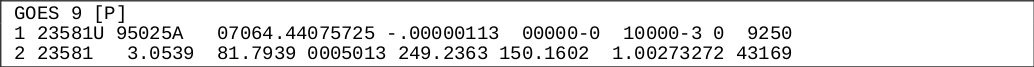
\includegraphics[scale=0.35]{fig/example_of_tle}
\caption{Example of Two Line Element Set (TLE)}
\label{fig:Example of Two Line Element Set (TLE)}
\end{figure}

Although TLEs are the most common format in which satellite orbit data may be received (for example, via NORAD or CelesTrak), it is recommended to instead use the CCSDS OMM format (as introduced in the following) when generating or further distributing such information. One reason for this is that while TLE inherently uses SGP4 models for most earth orbiting satellites, the OMM format allows for explicit definition of which propagation algorithm to use.

\begin{tabular}{l}
\textit{CCSDS 500.0-G "Navigation Data — Definitions and Conventions" \cite{CCSDS 500.0-G}} \\
\end{tabular}

This report contains technical material to supplement the following standards for spacecraft navigation data. The topics covered include radiometric data content, spacecraft ephemeris, planetary ephemeris, tracking station locations, coordinate systems, and attitude data. 

\begin{tabular}{l}
\textit{CCSDS 502.0-B "Orbit Data Messages" \cite{CCSDS 502.0-B}} \\
\end{tabular}

This standard specifies message formats for use in transferring spacecraft orbit information. Namely it defines three different orbit data message formats:

\begin{itemize}
\item Orbit parameter message (OPM): specifies the position and velocity of a single object at a specified epoch. It requires the use of a propagation technique to determine position and velocity at times different from the epoch.
\item Orbit mean-elements message (OMM): specifies the orbital characteristics of a single object at a specified epoch, expressed in mean Keplerian elements. It can be used to convert to and from TLE messages. Figure \ref{fig:Example of Orbit Mean-Elements Message (OMM)} shows the corresponding OMM for the TLE shown in \ref{fig:Example of Two Line Element Set (TLE)}.
\item Orbit ephemeris message (OEM): specifies the position and velocity of a single object at multiple epochs contained within a specified time range. It is well suited for automated interaction and allows for higher precision compared to the other formats. It requires the use of an interpolation technique to interpret the position and velocity at times different from the tabular epochs. 
\end{itemize}

\begin{figure}[h]
\centering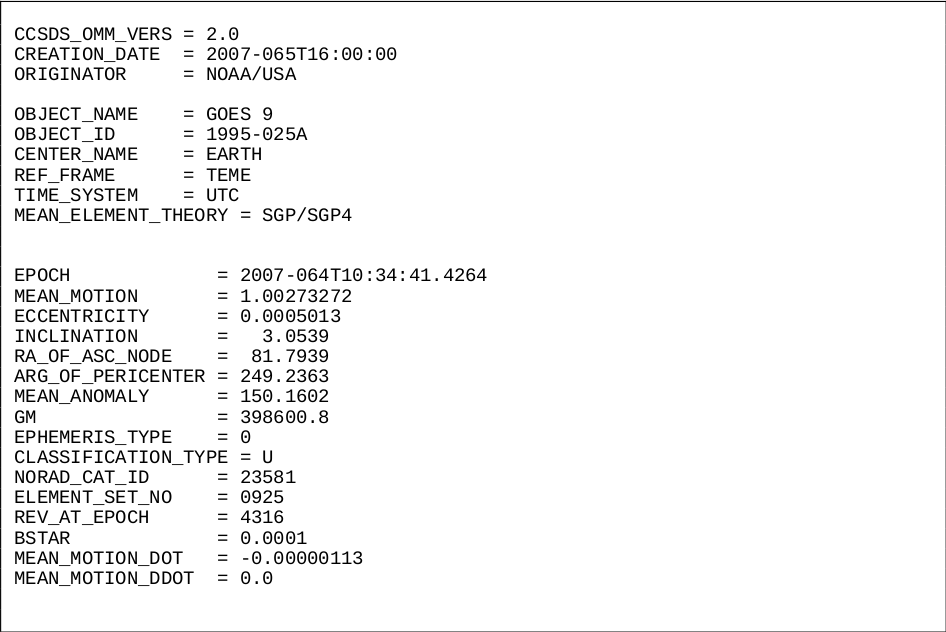
\includegraphics[scale=0.35]{fig/example_of_omm}
\caption{Example of Orbit Mean-Elements Message (OMM)}
\label{fig:Example of Orbit Mean-Elements Message (OMM)}
\end{figure}

\begin{tabular}{l}
\textit{CCSDS 503.0-B "Tracking Data Message" \cite{CCSDS 503.0-B}} \\
\end{tabular}

This standard specifies a message format for use in exchanging of spacecraft tracking data, that is data pertinent to a ground station tracking a satellite. Tracking data includes data types such as Doppler, transmit/receive frequencies, range, ground antenna pointing angles, weather (at station), etc. The message format is suitable for automated interaction.

\begin{tabular}{l}
\textit{CCSDS 504.0-B "Attitude Data Message" \cite{CCSDS 504.0-B}} \\
\end{tabular}

This standard specifies message formats for use in transferring spacecraft orbit information. Namely it defines two different attitude data message formats:

\begin{itemize}
\item Attitude parameter message (APM): specifies the attitude state of a single object at a specified epoch. It requires the use of a propagation technique to determine the attitude state at times different from the epoch.
\item Attitude ephemeris message (AEM): specifies the attitude state of a single object at multiple epochs contained within a specified time range. It is well suited for automated interaction and allows for higher precision. It requires the use of an interpolation technique to interpret the attitude state at times different from the tabular epochs. 
\end{itemize}

\begin{tabular}{l}
\textit{CCSDS 505.0-B "XML Specification for Navigation Data Messages" \cite{CCSDS 505.0-B}} \\
\end{tabular}

This standard describes an integrated XML schema set suited for exchanges of above navigation data messages . 

\begin{tabular}{l}
\textit{CCSDS 508.0-B "Conjunction Data Message" \cite{CCSDS 508.0-B}} \\
\end{tabular}

This standard specifies a message format for use in exchange of spacecraft conjunction information between originators of conjunction assessments and satellite owner/operators and other authorized parties. 

\begin{tabular}{l}
\textit{CCSDS 509.0-B "Pointing Request Message" \cite{CCSDS 509.0-B}} \\
\end{tabular}

This standard defines a message format to allow exchange of information about a requested pointing of a spacecraft. These can be requested (sequences of) changes of the attitude of the spacecraft or of an articulate spacecraft component. Pointing requests are transmitted, for instance, from scientists who operate an onboard instrument to the operator of the  spacecraft.
  
\subsection{Simulator}

\begin{tabular}{l}
\textit{ECSS-E-TM-10-21 "System modeling and simulation" \cite{ECSS-E-TM-10-21}} \\
\end{tabular}

Simulation is conducted to support the analysis, design, and verification activities of a space system. Simulation during analysis and design is usually carried out with simplified that then become more and more complex. During development, these software models are partly exchanged with real hardware, to do hardware-in-the-loop testing. During mission operations phase then, the simulation integrates high-fidelity models of the spacecraft and its environment, and possibly uses emulators to run the flight software within the simulation environment.

A simulator is composed of all or a subset of the components shown in Figure \ref{fig:Simulator Components}.

\begin{figure}[h]
\centering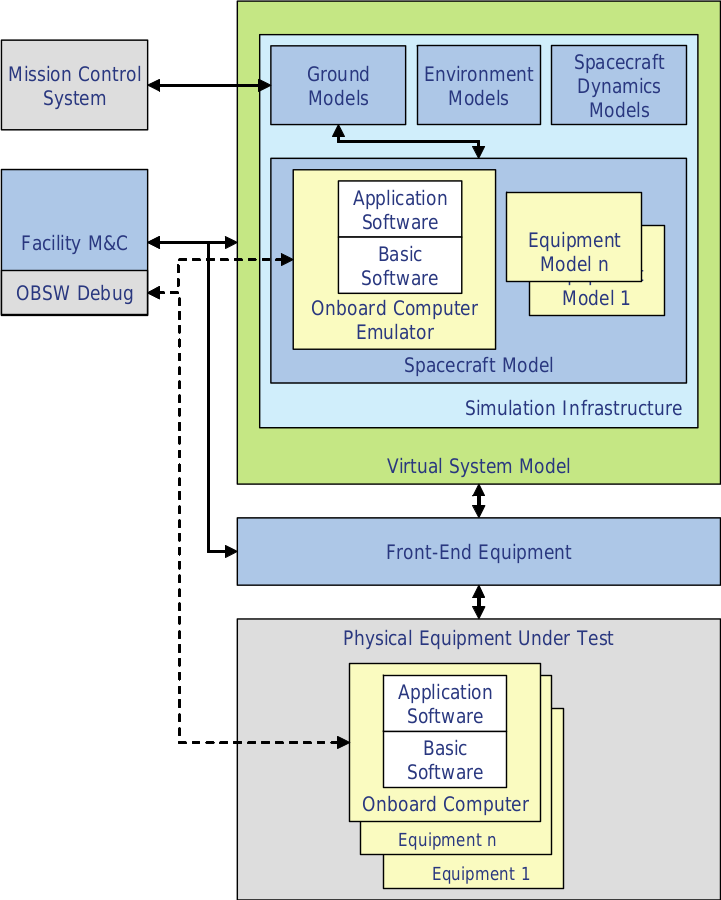
\includegraphics[scale=0.45]{fig/simulator_components}
\caption{Simulator Components}
\label{fig:Simulator Components}
\end{figure}

\begin{tabular}{l}
\textit{ECSS-E-TM-40-07 "System modelling platform - Volume 1 to 5" \cite{ECSS-E-TM-40-07}} \\
\end{tabular}

The virtual system model shown in Figure \ref{fig:Simulator Components} is composed of many simulation models that are part of the simulation infrastructure. Although those models simulate different aspects, such as ground models or the space environment, they often can be reused for various missions. The same applies to the spacecraft model, which is composed of various lower level models, some of which may have already be used on other missions. 

To ease portability and allow reuse of simulation models, the simulation modelling platform (SMP) was established that defines a simulation model definition language (SMDL) to allow platform independent design of models in terms of catalogs, integrate those as assemblies, and schedule them (Figure \ref{fig:SMP Overview}). 

\begin{figure}[h]
\centering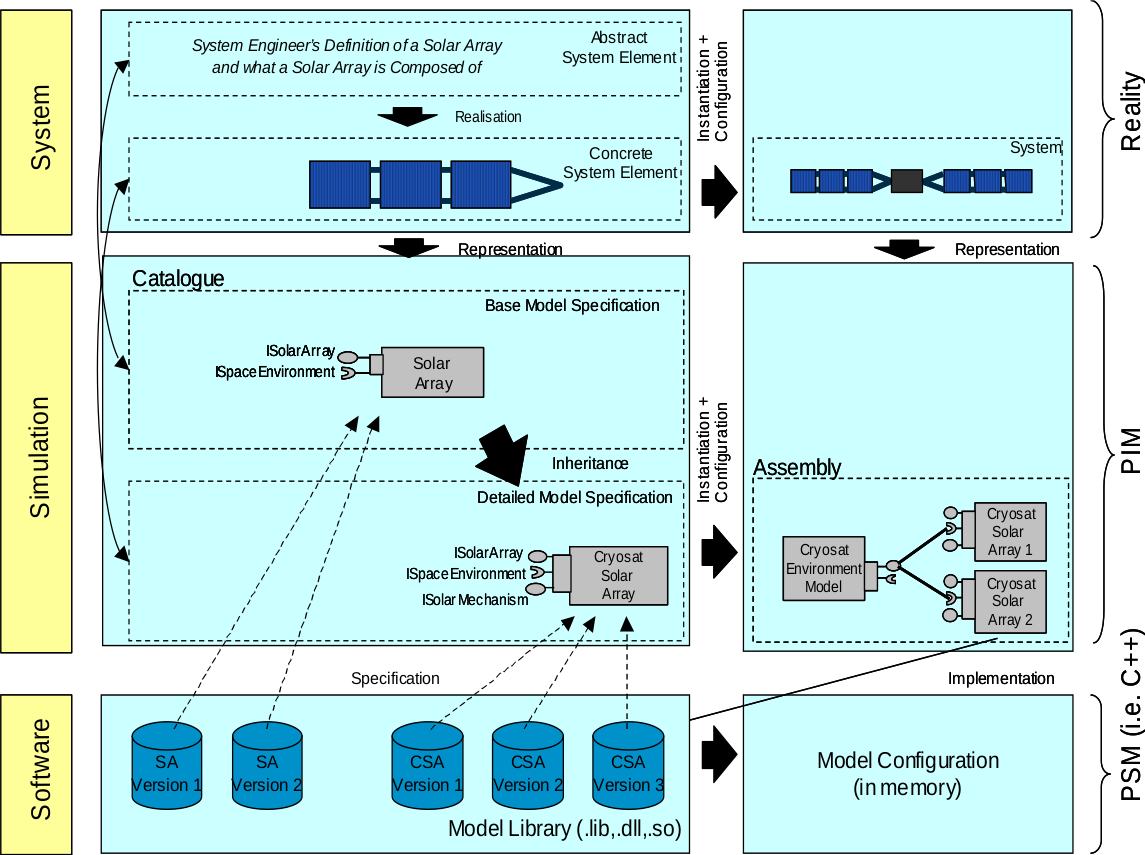
\includegraphics[scale=0.35]{fig/smp_overview}
\caption{SMP Overview}
\label{fig:SMP Overview}
\end{figure}

The SMP defines a generic pattern for component models, including a set of mandatory interfaces that each model has to implement. Further, the simulator services itself are defined (Figure \ref{fig:SMP Architecture}).

\begin{figure}[h]
\centering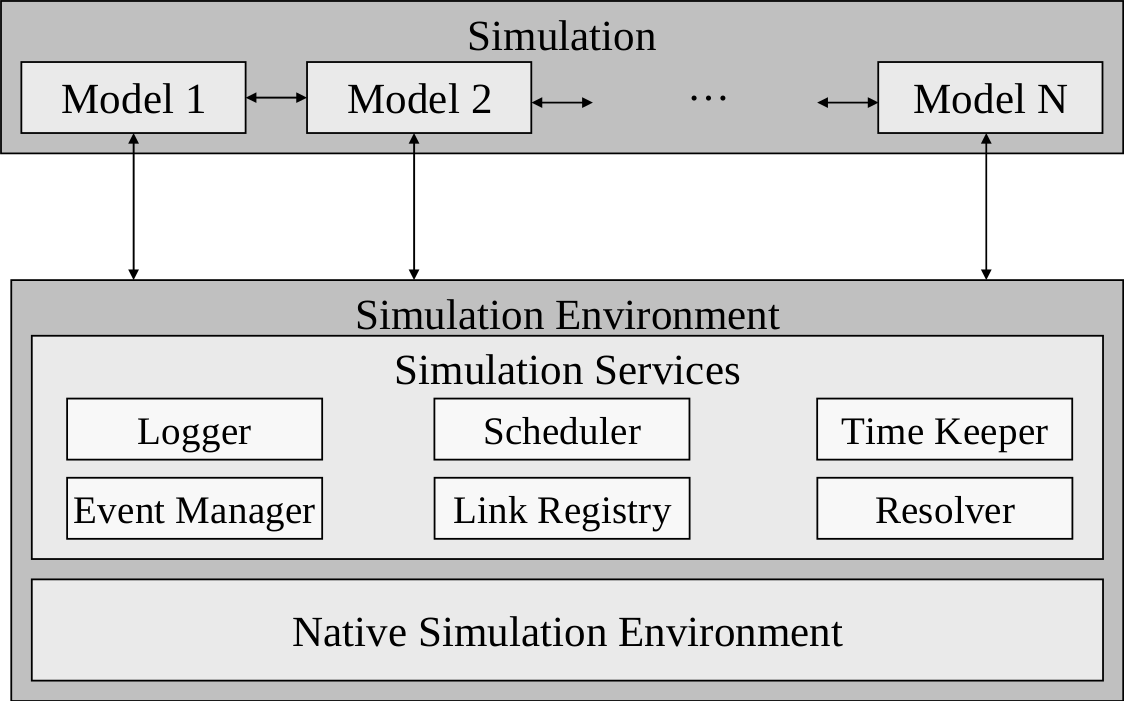
\includegraphics[scale=0.3]{fig/smp_architecture}
\caption{SMP Architecture}
\label{fig:SMP Architecture}
\end{figure}
